\documentclass[12pt]{article}

\usepackage{amsmath}
\usepackage{amsfonts}
\usepackage{float}
\usepackage{fancyhdr}
\usepackage{graphicx}
\usepackage[colorlinks=true,linkcolor=blue, citecolor=red]{hyperref}
\usepackage[table,xcdraw]{xcolor}
\usepackage{url}
\usepackage[top=.75in, left=.75in, right=.75in, bottom=1in]{geometry}
\usepackage[utf8]{vietnam}

% For algorithm
\usepackage{algorithm}
\usepackage{algpseudocode}

% ============ CODE ============
\usepackage{listings}
\usepackage{xcolor}
\definecolor{codegreen}{rgb}{0,0.6,0}
\definecolor{codegray}{rgb}{0.5,0.5,0.5}
\definecolor{codepurple}{rgb}{0.58,0,0.82}
\definecolor{backcolour}{rgb}{0.95,0.95,0.92}

% Styling for the code.
\lstdefinestyle{mystyle}{
    backgroundcolor=\color{backcolour},   
    commentstyle=\color{codegreen},
    keywordstyle=\color{magenta},
    numberstyle=\tiny\color{codegray},
    stringstyle=\color{codepurple},
    basicstyle=\ttfamily\footnotesize,
    breakatwhitespace=false,         
    breaklines=true,                 
    captionpos=b,                    
    keepspaces=true,                 
    numbers=left,                    
    numbersep=5pt,                  
    showspaces=false,                
    showstringspaces=false,
    showtabs=false,                  
    tabsize=2
}
\lstset{style=mystyle}

% Disable indentation on new paragraphs
\setlength{\parindent}{0pt}

% Optional: graphic path
% \graphicspath{PATH_TO_GRAPHIC_FOLDER}

% To use Times font family, uncomment this row
% \usepackage{mathptmx}

% To use roman section / subsection, uncomment these rows
% \renewcommand{\thesection}{\Roman{section}}
% \renewcommand{\thesubsection}{\thesection.\Roman{subsection}}

% Define course name, report name and report title.
\newcommand{\coursename}{Academic Proficiency Test - VNUHCM 2024}
\newcommand{\reportname}{Kì thi Đánh giá năng lực ĐHQG-HCM năm 2024}
\newcommand{\reporttitle}{Hướng dẫn Ôn tập}

\newcommand{\studentname}{Đinh Đức Tài (TK9-CBL)}
\newcommand{\teachername}{TK9.cbl}

\newcommand{\leftfooter}{\LaTeX\ by \href{https://facebook.com/ductai05}{Đinh Đức Tài}}

% ============ HEADER AND FOOTER ============
% Header length
\setlength{\headheight}{29.43912pt}

% Footer page number would be on the lower-right corner
\pagestyle{fancy}
\fancyfoot{}
\fancyfoot[R]{Trang \thepage}

\lhead{\reporttitle}
\rhead{
Đánh giá năng lực - ĐHQG TP.HCM 2024\\
\coursename
}
\lfoot{\leftfooter}

% ============ DOCUMENT ============
\begin{document}
\begin{titlepage}
\newcommand{\HRule}{\rule{\linewidth}{0.5mm}}
\centering

\textsc{\LARGE chuyên toán, khóa 9 \\trường thpt chuyên bảo lộc}\\[1.5cm]

\HRule \\[0.4cm]
{ 
\huge{\bfseries{\reporttitle}}\\[0.5cm]
\large{\bfseries{\reportname}}
}\\[0.4cm]
\HRule \\[0.5cm]

\textbf{\large \coursename}\\[0.5cm]

\begin{minipage}[t]{0.4\textwidth}
\begin{flushleft} \large
\emph{Tác giả:}\\
\studentname
\end{flushleft}
\end{minipage}
~
\begin{minipage}[t]{0.4\textwidth}
\begin{flushright} \large
\emph{Cố vấn:} \\
\teachername
\end{flushright}
\end{minipage}\\[2cm]

{\large \today}\\[3cm]


\includegraphics[scale=.12]{img/cbl_tk9.jpg}\\[1cm] 

\vfill
\end{titlepage}
	
	
\tableofcontents
\pagebreak


\section{Giới thiệu}
\begin{itemize}
    \item Đây là \textbf{tài liệu tổng hợp thông tin} và \textbf{hướng dẫn ôn tập}, hướng đến \textbf{kỳ thi ĐGNL ĐHQG-HCM năm 2024}. Thân gửi các bạn học sinh 2006, đặc biệt là Khóa 10, trường THPT Chuyên Bảo Lộc.
\end{itemize}
\section{Kỳ thi Đánh giá năng lực ĐHQG-TPHCM}
\subsection{Tổng quan kỳ thi}
\subsubsection{Mục tiêu}
\begin{itemize}
    \item \textbf{Bài thi ĐGNL ĐHQG-HCM} chú trọng đánh giá các năng lực cơ bản để học đại học của thí sinh: sử dụng ngôn ngữ, tư duy logic, xử lý số liệu, giải quyết vấn đề. Về hình thức, bài thi gồm \textbf{120 câu hỏi trắc nghiệm} khách quan đa lựa chọn với \textbf{thời gian làm bài 150 phút}.
    \item \textbf{Về nội dung}, đề thi cung cấp số liệu, dữ kiện và các công thức cơ bản nhằm đánh giá khả năng suy luận và giải quyết vấn đề, \textbf{không đánh giá khả năng học thuộc lòng}. 
    \item Đề thi được xây dựng cùng cách tiếp cận như đề thi SAT (Scholastic Assessment Test) của Hoa kỳ và đề thi TSA (Thinking Skills Assessment) của Anh
\end{itemize}

\subsubsection{Danh sách các đơn vị xét tuyển bằng kết quả Kỳ thi ĐGNL 2024}
\begin{itemize}
    \item Các \textbf{đơn vị xét tuyển} bằng kết quả kì thi ĐGNL 2024 gồm các trường \textbf{trong ĐHQG-HCM} và các đại học và trường đại học \textbf{ngoài ĐHQG-HCM} (UDN, UEH, NEU, UAH, ...). \cite{dvxettuyen}
    \item Ngoài ra thí sinh còn có thể sử dụng điểm ĐGNL của ĐHQG-HCM (APT) để \textbf{quy đổi} ra điểm ĐGNL của ĐHQG-HN (HSA) theo công thức: \texttt{HSA = 0,1103 x APT}. \cite{apt_to_hsa} 
\end{itemize}
 
\subsubsection{Các mốc thời gian, địa điểm thi} 
Các bạn học sinh \textbf{có thể đăng kí thi cả hai đợt ĐGNL ở Lâm Đồng} \cite{thoigian_diadiem} (so với khóa trước thì Đợt 2 không tổ chức ở Lâm Đồng mà phải xuống TP.HCM để thi)
\begin{enumerate}
    \item \textbf{Đợt 1: Ngày 07/04/2024}
    \begin{itemize}
        \item 22/01/2024: Mở đăng ký dự thi ĐGNL đợt 1
        \item 04/3/2024: Kết thúc đăng ký dự thi ĐGNL đợt 1
        \item \textbf{07/4/2024: Tổ chức thi ĐGNL đợt 1 tại 24 tỉnh/thành phố gồm:}
        \begin{itemize}
            \item Trung và Nam Trung Bộ: Thừa Thiên Huế, Đà Nẵng, Quảng Nam, Quảng Ngãi, Bình Định, Phú Yên, Khánh Hòa, Bình Thuận
            \item Tây Nguyên: Đắk Lắk, \textbf{Lâm Đồng - Trường ĐH Đà Lạt}
            \item Đông Nam Bộ: Thành phố Hồ Chí Minh, Bình Dương, Đồng Nai, Bà Rịa – Vũng Tàu, Bình Phước và Tây Ninh
            \item Tây Nam Bộ: Tiền Giang, Bến Tre, Đồng Tháp, Vĩnh Long, An Giang, Cần Thơ, Kiên Giang, Bạc Liêu
        \end{itemize}
        \item 15/4/2024: Thông báo kết quả thi ĐGNL đợt 1.
    \end{itemize}
    \item \textbf{Đợt 2: Ngày 02/6/2024}
    \begin{itemize}
        \item 16/4/2024: Mở đăng ký dự thi ĐGNL đợt 2
        \item 07/5/2024: Kết thúc đăng ký dự thi ĐGNL đợt 2
        \item \textbf{02/6/2024: Tổ chức thi ĐGNL đợt 2 tại 12 tỉnh/thành phố gồm:}
        \begin{itemize}
            \item Trung và Nam Trung Bộ: Thừa Thiên Huế, Đà Nẵng, Bình Định, Khánh Hòa
            \item Tây Nguyên: Đắk Lắk, \textbf{Lâm Đồng}
            \item Đông Nam Bộ: Thành phố Hồ Chí Minh, Bà Rịa- Vũng Tàu, Đồng Nai, Bình Dương
            \item Tây Nam Bộ: Tiền Giang, An Giang
        \end{itemize}
        \item 10/6/2024: Thông báo kết quả thi ĐGNL đợt 2
    \end{itemize}
\end{enumerate}

\subsection{Các trang web liên quan đến kì thi}
\begin{itemize}
    \item \textbf{Cổng thông tin đăng kí:} \href{https://thinangluc.vnuhcm.edu.vn/dgnl/}{https://thinangluc.vnuhcm.edu.vn/dgnl/} \cite{webdangki}
    \item Các bạn nên tham khảo các thông tin trên website của Trung tâm khảo thí và Đánh giá chất lượng đào tạo ĐHQG-HCM: \href{http://cete.vnuhcm.edu.vn/thi-danh-gia-nang-luc.html}{http://cete.vnuhcm.edu.vn/thi-danh-gia-nang-luc.html} \cite{cetevnuhcm}
\end{itemize}

\subsection{Cấu trúc bài thi ĐGNL}
\label{cautrucbaithi}
Cấu trúc của bài thi ĐGNL gồm \textbf{3 phần}: Sử dụng ngôn ngữ; Toán học, tư duy logic và
phân tích số liệu; và Giải quyết vấn đề.
\subsubsection{Phần 1. Sử dụng ngôn ngữ (40 câu)}
\paragraph{a) Tiếng Việt (20 câu):}Đánh giá năng lực đọc hiểu văn bản và sử dụng tiếng Việt, và khả năng cảm thụ, phân tích các tác phẩm văn học. Đề thi tích hợp nhiều kiến thức về ngữ văn, đòi hỏi thí sinh nắm vững những kỹ năng thực hành tiếng Việt để áp dụng vào giải quyết các vấn đề liên quan.
\par

\begin{table}[H]
\begin{tabular}{|l|l|}
\hline
\textbf{Nội dung đánh giá} & \textbf{Mô tả} \\ \hline
Hiểu biết văn học & \begin{tabular}[c]{@{}l@{}}Đánh giá khả năng hiểu các kiến thức văn học cơ bản như: phong cách\\ sáng tác của các tác giả tiêu biểu, nội dung và hình thức nghệ thuật của \\ tác phẩm; vai trò của tác giả, tác phẩm đối với lịch sử văn học.\end{tabular} \\ \hline
Sử dụng tiếng Việt & \begin{tabular}[c]{@{}l@{}}Đánh giá khả năng nhận biết vấn đề về sử dụng tiếng Việt như: xác định \\ những từ viết không đúng quy tắc chính tả, những từ sử dụng sai, những \\ câu mắc lỗi ngữ pháp diễn đạt; nhận biết cấu tạo từ, các biện pháp tu từ, \\ các vấn đề thuộc về ngữ pháp câu, các thành phần trong câu, phép liên \\ kết câu,…\end{tabular} \\ \hline
Đọc hiểu văn bản & \begin{tabular}[c]{@{}l@{}}Đánh giá khả năng phân loại đặc trưng phong cách (phong cách thể loại, \\ phong cách tác giả, phong cách chức năng ngôn ngữ, …), xác định ý \\ nghĩa của từ/câu trong văn bản, cách tổ chức văn bản, các thủ pháp nghệ \\ thuật được sử dụng, nội dung và tư tưởng của văn bản.\end{tabular} \\ \hline
\end{tabular}
\end{table}

\paragraph{b) Tiếng Anh (20 câu):}Đánh giá năng lực sử dụng tiếng Anh tổng quát ở cấp độ A2-B1 theo khung năng lực ngoại ngữ 6 bậc, thông qua các nội dung: lựa chọn cấu trúc câu, nhận diện lỗi sai, đọc hiểu câu, đọc hiểu đoạn văn:
\par

\begin{table}[H]
\begin{tabular}{|l|l|}
\hline
\textbf{Nội dung đánh giá} & \textbf{Mô tả} \\ \hline
Lựa chọn cấu trúc câu & \begin{tabular}[c]{@{}l@{}}Đánh giá khả năng hiểu và áp dụng các cấu trúc câu thông qua việc \\ yêu cầu thí sinh chọn từ/cụm từ có cấu trúc phù hợp để điền vào \\ khoảng trống.\end{tabular} \\ \hline
Nhận diện lỗi sai & \begin{tabular}[c]{@{}l@{}}Đánh giá khả năng hiểu các kiến thức ngữ pháp và áp dụng để giải\\ quyết vấn đề thông qua việc nhận diện lỗi sai trong những phần \\ được gạch chân.\end{tabular} \\ \hline
Đọc hiểu câu & \begin{tabular}[c]{@{}l@{}}Đánh giá khả năng đọc hiểu câu và khả năng áp dụng kiến thức ngữ\\ pháp đã học thông qua việc chọn câu có nghĩa gần nhất với \\ câu đã cho.\end{tabular} \\ \hline
Đọc hiểu đoạn văn & \begin{tabular}[c]{@{}l@{}}Đánh giá khả năng hiểu và áp dụng kiến thức ngữ pháp cũng như \\ kỹ năng đọc lướt để lấy thông tin (skimming) và đọc kỹ để tìm chi \\ tiết (scanning), cụ thể: đọc lướt để trả lời câu hỏi lấy ý chính (main \\ idea), đọc kỹ để trả lời các câu hỏi tham chiếu (reference), câu hỏi \\ chi tiết (detail), câu hỏi từ vựng (vocabulary), câu hỏi suy luận \\ (inference).\end{tabular} \\ \hline
\end{tabular}
\end{table}

\subsubsection{Phần 2. Toán học, tư duy logic và phân tích số liệu (30 câu)}
\paragraph{}Đánh giá khả năng áp dụng các kiến thức toán học; khả năng tư duy logic; khả năng diễn giải, so sánh phân tích số liệu:
\par

\begin{table}[H]
\begin{tabular}{|l|l|}
\hline
\textbf{Nội dung đánh giá} & \textbf{Mô tả} \\ \hline
Toán học & \begin{tabular}[c]{@{}l@{}}Đánh giá khả năng hiểu và áp dụng các kiến thức toán học trong chương \\ trình giáo khoa trung học phổ thông thuộc các nội dung: ứng dụng của \\ đạo hàm để khảo sát hàm số, số phức (tìm phần thực, phần ảo Mô-đun, \\ không có phương trình bậc 2, không có dạng lượng giác), hình học thuần \\ túy, hình học tọa độ, tích phân và ứng dụng của tích phân, tổ hợp và xác \\ suất, hàm số logarit, giải toán bằng cách lập hệ phương trình, giải hệ \\ phương trình tuyến tính suy biến.\end{tabular} \\ \hline
Tư duy logic & \begin{tabular}[c]{@{}l@{}}Đánh giá khả năng suy luận logic thông qua các hình thức logic đơn lẻ \\ và nhóm logic tình huống. Dựa vào các thông tin được cung cấp trong \\ mỗi tình huống logic cùng với kỹ năng suy luận và phân tích, thí sinh \\ tìm phương án khả thi cho các giả định được đưa ra.\end{tabular} \\ \hline
Phân tích số liệu & \begin{tabular}[c]{@{}l@{}}Đánh giá khả năng đọc và phân tích số liệu thực tế thông qua các sơ đồ \\ và các bảng số liệu. Các sơ đồ và bảng biểu xuất hiện trong đề thi gồm: \\ biểu đồ tròn, biểu đồ Venn, biểu đồ cột, biểu đồ đường, biểu đồ dạng \\ bảng số liệu.\end{tabular} \\ \hline
\end{tabular}
\end{table}

\subsubsection{Phần 3. Giải quyết vấn đề (50 câu)}
\paragraph{}Đánh giá khả năng hiểu các kiến thức giáo khoa cơ bản và áp dụng để giải quyết các vấn đề cụ thể thuộc năm lĩnh vực, gồm ba lĩnh vực khoa học tự nhiên (hóa học, vật lý, sinh học) và hai lĩnh vực khoa học xã hội (địa lí, lịch sử):
\par

\begin{table}[H]
\begin{tabular}{|l|l|}
\hline
\textbf{Nội dung đánh giá} & \textbf{Mô tả} \\ \hline
\begin{tabular}[c]{@{}l@{}}Lĩnh vực khoa học tự nhiên \\ (hóa học, vật lí, sinh học)\end{tabular} & \begin{tabular}[c]{@{}l@{}}Các câu hỏi đơn lẻ đánh giá khả năng hiểu các kiến thức giáo khoa \\ cơ bản liên quan đến ba lĩnh vực khoa học tự nhiên: hóa học, vật lý, \\ sinh học.\\ Các nhóm câu hỏi tình huống đánh giá khả năng đọc, tư duy, suy \\ luận logic về hóa học, vật lí, sinh học thông qua dữ kiện được cung \\ cấp trong các bài đọc và kiến thức đã học; đánh giá khả năng áp \\ dụng các kiến thức phổ thông để giải quyết các vấn đề liên quan.\end{tabular} \\ \hline
\begin{tabular}[c]{@{}l@{}}Lĩnh vực khoa học xã hội \\ (địa lí, lịch sử)\end{tabular} & \begin{tabular}[c]{@{}l@{}}Các câu hỏi đơn lẻ đánh giá khả năng  hiểu kiến thức giáo khoa cơ \\ bản liên quan đến lĩnh vực khoa học xã hội: địa lý, lịch sử.\\ Các nhóm câu hỏi tình huống đánh giá khả năng đọc, tư duy, suy \\ luận logic về địa lý, lịch sử thông qua dữ kiện được cung cấp \\ trong các bài đọc, kiến thức đã học hoặc kiến thức thực tế; \\ năng lực áp dụng các kiến thức phổ thông để giải quyết các \\ vấn đề liên quan.\end{tabular} \\ \hline
\end{tabular}
\end{table}



\section{Tổng quan quá trình Học và Giải đề ĐGNL}
\subsection{Kiến thức căn bản}\label{sec:basic}
Đối với các kiến thức căn bản, các bạn xem kĩ hơn ở phần 4: \hyperref[sec:bigbasic]{Kiến thức căn bản}
\\Các lĩnh vực chính: Tiếng Việt, Tiếng Anh, Toán, Khoa học tự nhiên, Khoa học xã hội.
\subsection{Giải đề}
\subsubsection{Lưu ý}

\paragraph{Đôi lời về bộ đề ĐGNL và việc giải đề}

\begin{itemize}
    \item Trong bộ đề gồm 20 đề - tức là rất nhiều. Mục đích của các bạn \textbf{không phải là làm hết 20 đề} này.
    \item \textbf{Bước 1:} Các bạn nên làm 1 đến 2 đề (hoặc làm đề mẫu năm 2024 \cite{demau2024}) với mục đích \textbf{tìm giới hạn  \hyperref[sec:phamvikienthuc]{phạm vi kiến thức}} mà đề sẽ hỏi. 
    \item \textbf{Bước 2:} \textbf{học và nắm chắc phần kiến thức} này.
    \item \textbf{Bước 3:} Giải đề để \textbf{nâng cao \hyperref[sec:kinanglambai]{kĩ năng}} làm bài thi. Có thể lặp lại từ bước 1.
    \item \textbf{Lưu ý:} Chỉ giải đề khi đã có lượng kiến thức căn bản nhất định (hãy nắm chắc \hyperref[sec:basic]{Kiến thức căn bản} trước). 
\end{itemize}

\subsubsection{Kĩ thuật giải đề}
\textbf{Luyện tập thông thường:} Các bạn có thể chuyển qua \hyperref[sec:giaidephongthi]{Luyện tập giải đề trong phòng thi} hoặc theo các bước sau:

\begin{enumerate}
    \item Sử dụng \href{https://www.example.com}{Bộ đề ôn thi ĐGNL} \cite{bo_de_thidgnl}
    \item \textbf{Giải đề} và đánh dấu lại đáp án.
    \item Mở đáp án của bộ đề, \textbf{chấm điểm, ghi chú} lại những kiến thức còn thiếu hoặc làm sai. 
    \item Cố gắng nâng cao thành tích trong những bộ đề sau.
\end{enumerate}
\begin{figure}[H]
    \centering
    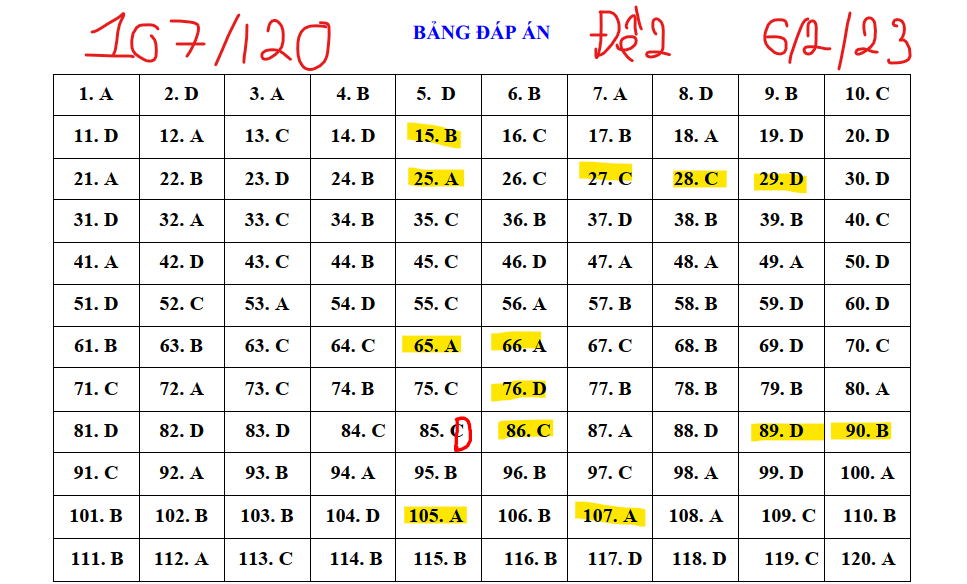
\includegraphics[width=1\linewidth]{img/Đề 2 -107_120.png}
    \caption{Đối chiếu đáp án và chấm điểm}
    \label{fig:giaidethu}
\end{figure}

\paragraph{Luyện tập giải đề trong phòng thi:}\label{sec:giaidephongthi}
\begin{enumerate}
    \item Sử dụng \href{https://www.example.com}{Bộ đề ôn thi ĐGNL} \cite{bo_de_thidgnl}
    \item Tải \href{https://drive.google.com/file/d/1IhtAQb20qTUOxD3zjC1bvKnkarBYnSok/view?usp=drive_link}{Phiếu A4 - 120 câu} \cite{phieuA4} và in trên tờ A4 (tờ trả lời trắc nghiệm).
    \item Tải app \href{https://play.google.com/store/apps/details?id=com.quiz.marker}{Chấm thi trắc nghiệm} \cite{appchamthi} \footnote{Có thể bạn chưa biết: Các thầy cô cũng dùng một ứng dụng tương tự trên điện thoại để chấm bài thi học kì (trắc nghiệm).}
    \item Mở bảng đáp án của đề sắp giải, \textbf{điền các đáp án vào phần mềm}.
    \item Cài đặt bộ đếm giờ, \textbf{reset lại não} (để quên đáp án vừa nãy nhìn) và làm bài. \textbf{Điền đáp án trực tiếp vào tờ trả lời trắc nghiệm}.
    \item Sau khi làm bài, \textbf{dùng app} để quét tờ trắc nghiệm. 
    \item \textbf{Chấm điểm, ghi chú} lại những kiến thức còn thiếu hoặc làm sai. 
    \item Cố gắng nâng cao thành tích trong những bộ đề sau.
\end{enumerate}
\begin{figure}[H]
    \centering
    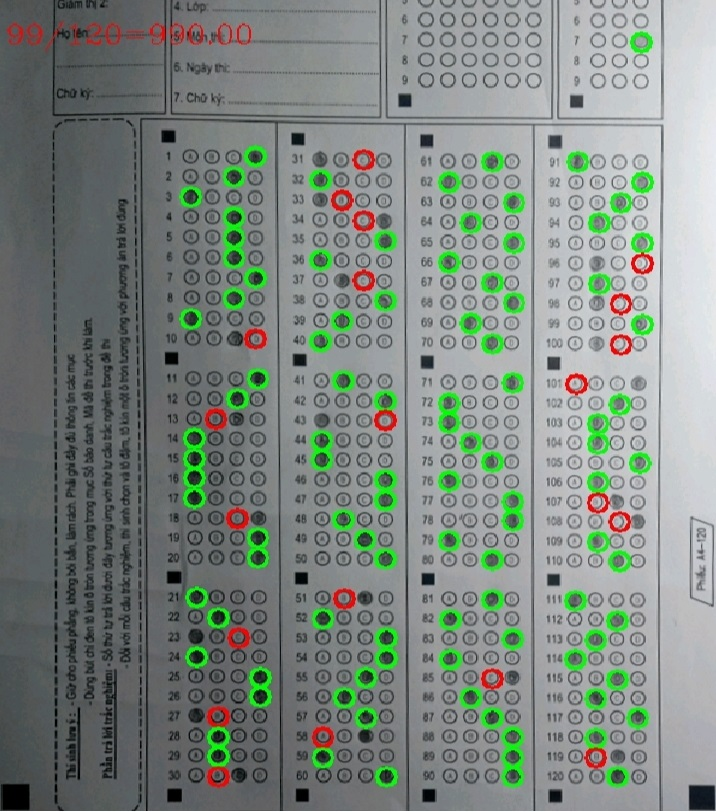
\includegraphics[width=0.7\linewidth]{img/cham_bang_app.jpg}
    \caption{Tô trắc nghiệm lên giấy và chấm bằng app}
    \label{fig:chambângppp}
\end{figure}



\newpage
\section{Kiến thức và kĩ năng}
\label{sec:bigbasic}

\subsection{Cấu trúc bài thi, gợi ý cách học}
\label{sec:goiycachhoc}
\textbf{Về cấu trúc bài thi:}
\begin{itemize}
    \item Các bạn nên xem lại \textbf{\hyperref[cautrucbaithi]{cấu trúc bài thi ĐGNL}}.
    \item \textbf{Phân bố điểm} trong bài thi: \textbf{Tiếng Việt (20 câu)}, \textbf{Tiếng Anh (20 câu)}, \textbf{Toán học, logic, phân tích số liệu (30 câu)}, \textbf{Khoa học tự nhiên (Vật lí, Hóa học, Sinh học mỗi phần 10 câu)}, \textbf{Khoa học xã hội (Địa lí, Lịch sử mỗi phần 10 câu)}
    \item Có thể thấy: \textbf{Toán học} và \textbf{Khoa học tự nhiên} chiếm \textbf{trọng số cao} hơn trong bài thi so với \textbf{Khoa học xã hội} (lí do là phân môn GDCD không được đưa vào bài thi ĐGNL). Vì vậy lời khuyên cho các bạn học khối xã hội là \textbf{nên cải thiện về mảng Toán và Khoa học tự nhiên} (rất quan trọng nhé).
    \item Về phần \textbf{ngôn ngữ} (tiếng Việt, tiếng Anh): Phạm vi câu hỏi của tiếng Việt rất rộng. Các bạn nên đọc thêm về \textbf{ca dao, tục ngữ Việt Nam} và các \textbf{lỗi chính tả} thường gặp. Với tiếng Anh, các bạn có trình độ \textbf{B1 - B2} (IELTS 4.5 - 5.5) sẽ là khá ổn để làm bài thi.
    \item Về phần \textbf{Khoa học xã hội}, các bạn nên \textbf{chú ý nghe giảng trên lớp} \footnote{Đi du lịch Taiwan bằng tàu điện cao tốc 300km/h} để tiết kiệm thời gian học. Độ khó của phần Khoa học xã hội sẽ ngang với mức học trên lớp.
\end{itemize}
\textbf{Về các đợt thi:}
\begin{itemize}
     \item Đối với thi ĐGNL \textbf{Đợt 1}, trong đề sẽ có các câu hỏi vượt qua tiến độ kiến thức các bạn đang học trên lớp. Vì thế, \textbf{học vượt} tiến độ chương trình trên lớp sẽ là một \textbf{lợi thế}. 
    \item Với \textbf{Đợt 2}, \textbf{độ khó của đề sẽ tăng lên} để cân bằng với các bạn chỉ thi Đợt 1 (các bạn thi Đợt 2 được ôn nhiều hơn). Vậy nên thật khó nếu muốn so sánh tham gia đợt thi nào sẽ có lợi hơn. Dù vậy, điều thường thấy là các bạn thi Đợt 2 sẽ có điểm cao hơn. Tuy nhiên, mình \textbf{khuyến khích các bạn thi Đợt 1} hoặc \textbf{cả hai đợt} (vì nếu chỉ thi Đợt 2 sẽ ảnh hướng tới việc thi tốt nghiệp THPT; ngoài ra một số trường chỉ xét Đợt 1).
\end{itemize}
\textbf{Gợi ý cách học:}
\begin{itemize}
    \item Mỗi bạn sẽ có phương pháp học tập \textbf{khác nhau}, hãy \textbf{tìm} và \textbf{lựa chọn phương pháp} phù hợp nhất. Dưới đây là một vài gợi ý:
    \item Học lệch sẽ kéo điểm bài thi xuống rất nhiều. Nên thay đổi hướng học để phù hợp với hướng xét tuyển đại học của các bạn (nếu \textbf{thi ĐGNL tuyệt đối không học lệch}).
    \item \textbf{Tập trung học trên lớp} sẽ giúp \textbf{tiết kiệm thời gian} ôn tập kiến thức.
    \item Không ai giỏi toàn bộ các môn nên phải \textbf{dành thời gian} nhiều hơn cho những \textbf{môn mình chưa vững}. 
    \item Bài thi sử dụng \textbf{câu hỏi ứng dụng} để đánh giá năng lực tư duy và đọc hiểu vấn đề. Nên tìm hiểu nhiều hơn các \textbf{kiến thức thực tế/bài tập hướng ứng dụng}.
    
\end{itemize}

\subsection{Phạm vi kiến thức}
\label{sec:phamvikienthuc}

\subsubsection{Tiếng Việt}
\begin{enumerate}
\item \textbf{Hiểu biết văn học}
    \begin{itemize}
        \item Phong cách sáng tác
        \item Nội dung, hình thức nghệ thuật
        \item Vai trò của tác giả, tác phẩm với lịch sử văn học
    \end{itemize}
\item \textbf{Sử dụng tiếng Việt}
    \begin{itemize}
        \item Chính tả
        \item Lỗi ngữ pháp diễn đạt
        \item Biện pháp tu từ
        \item Cấu tạo từ, các phần phần trong câu
        \item Phép liên kết câu
    \end{itemize}
\item \textbf{Đọc hiểu văn bản}
    \begin{itemize}
        \item Phân loại đặc trưng phong cách
        \item Xác định ý nghĩa của từ/câu trong văn bản
        \item Cách tổ chức văn bản
        \item Thủ pháp nghệ thuật
        \item Nội dung, tư tưởng văn bản
    \end{itemize}
\end{enumerate}
\subsubsection{Tiếng Anh}
\begin{enumerate}
    \item \textbf{Lựa chọn cấu trúc câu:} chọn \textbf{từ, cụm từ có cấu trúc phù hợp} để điền vào khoảng trống
    \item \textbf{Nhận diện lỗi sai:} nhận diện \textbf{lỗi sai} trong những phần được gạch chân
    \item \textbf{Đọc hiểu câu:} chọn câu có \textbf{nghĩa gần nhất} với câu đã cho
    \item \textbf{Đọc hiểu đoạn văn:} Hiểu, áp dụng kiến thức ngữ pháp, kỹ năng để: đọc \textbf{tìm ý} (skimming), \textbf{tìm chi tiết} (scanning), lấy \textbf{ý chính} (main idea); \textbf{trả lời câu hỏi} tham chiếu (reference), câu hỏi chi tiết (detail), câu hỏi từ vựng (vocabulary), câu hỏi suy luận (inference).
\end{enumerate}
\subsubsection{Toán, tư duy logic, phân tích số liệu}
\begin{enumerate}
    \item \textbf{Toán học}
    \begin{itemize}
        \item Ứng dụng đạo hàm để khảo sát hàm số
        \item Số phức
        \item Hình học thuần túy
        \item Hình học tọa độ Oxy, Oxyz
        \item Tích phân, ứng dụng tích phân
        \item Tổ hợp và xác suất
        \item Hàm số logarit
        \item Giải toán bằng cách lập hệ phương trình
        \item Giải hệ tuyến tính suy biến
    \end{itemize}
    
    \item \textbf{Tư duy logic}
    \begin{itemize}
        \item Logic đơn lẻ
        \item Logic nhóm tình huống
    \end{itemize}
    \item \textbf{Phân tích số liệu}
    \begin{itemize}
        \item Đọc và phân tích số liệu qua sơ đồ, bảng số liệu
        \item Biểu đồ tròn, biểu đồ Venn, biểu đồ cột, biểu đồ đường, biểu đồ dạng bảng số liệu
    \end{itemize}
\end{enumerate}
\begin{itemize}
    \item Tài liệu tham khảo: \href{https://www.nbv.edu.vn/2023/07/40-chuyen-de-2024.html}{https://www.nbv.edu.vn/2023/07/40-chuyen-de-2024.html} \\ \href{https://drive.google.com/drive/folders/1JBYkj8FNyg_dsuybkv0xJQ3jtTPyyFNL}{Tài liệu Toán}
\end{itemize}
\subsubsection{Khoa học tự nhiên}
\begin{enumerate}
    \item \textbf{Vật lý}
    \begin{itemize}
        \item Động học chất điểm, Động lực học chất điểm, Các định luật bảo toàn, Nhiệt động lực học, Chất rắn - lỏng - khí.
        \item Điện tích, \textbf{Điện - Từ trường}, Dòng điện, \textbf{Cảm ứng điện từ}, Khúc xạ ánh sáng, Mắt và dụng cụ quang học.
        \item \textbf{Dao động cơ}, \textbf{Sóng cơ và sóng âm}, \textbf{Dòng điện xoay chiều}, \textbf{Dao động và sóng điện từ}, \textbf{Sóng ánh sáng}, \textbf{Lượng tử ánh sáng}, \textbf{Hạt nhân nguyên tử}.
        \item Tài liệu tham khảo: SGK - SBT Vật lý 12 (chương trình cũ); \href{https://drive.google.com/drive/folders/1DDyPLypeOzVWsB3-JPDBNBk8See7p6g8}{Live C thầy Vũ Tuấn Anh}
    \end{itemize}
    \item \textbf{Hóa học}
    \begin{itemize}
        \item Nguyên tử, Bảng tuần hoàn, \textbf{Liên kết hóa học}, \textbf{Phản ứng Oxi hóa - khử}, Halogen, Oxi - Lưu huỳnh, \textbf{Tốc độ phản ứng và cân bằng hóa học}. 
        \item \textbf{Sự điện li}, Nito - Photpho, Cacbon - Silic, Hidrocacbon no - không no - thơm, \textbf{Dẫn xuất halogen - ancol - phenol}, Andehit - xeton - axit cacboxylic.
        \item \textbf{Este - Lipit}, \textbf{Cacbohidrat}, \textbf{Amin - Amino Axit - Protein}, \textbf{Polime}, \textbf{Kim loại - Kim loại kiềm, kiềm thổ, nhôm, sắt,...} \textbf{Hóa ứng dụng}.
        \item Tài liệu tham khảo: Tài liệu tham khảo: SGK - SBT Hóa học 12 (chương trình cũ); \href{https://drive.google.com/drive/folders/1ZuWHtl1ARV1sRz00ZvF_XRskvD9ggg_1}{Tài liệu Hóa}
    \end{itemize}
    \item \textbf{Sinh học}
    \begin{itemize}
        \item \textbf{Thế giới sống}, \textbf{Sinh học tế bào}, sinh học vi sinh vật
        \begin{itemize}
            \item Các cấp tổ chức của thế giới sống, Các giới sinh vật.
            \item Tế bào nhân sơ, nhân thực.
            \item \textbf{Nguyên phân}, \textbf{Giảm phân}.
        \end{itemize}
        \item \textbf{Sinh học cơ thể}
        \begin{itemize}
            \item \textbf{Chuyển hóa vật chất và năng lượng} ở thực vật và động vật.
            \item Cảm ứng ở thực vật và thực vật.
            \item \textbf{Sinh sản} ở thực vật và động vật.
        \end{itemize}
        \item \textbf{Di truyền học}, \textbf{Tiến hóa}, \textbf{Sinh thái học}
        \begin{itemize}
            \item Gen, nhân đôi ADN, \textbf{Phiên mã - dịch mã}, \textbf{Đột biến gen}, \textbf{NST và đột biến NST}.
            \item \textbf{Quy luật phân li - phân li độc lập}, \textbf{Tương tác gen}, \textbf{Liên kết - hoán vị gen}, Di truyền liên kết với giới tính, Di truyền ngoài nhân.
            \item Ứng dụng di truyền học: \textbf{biến dị tổ hợp}, đột biến, \textbf{công nghệ tế bào}, công nghệ gen.
            \item Di truyền học người: \textbf{bệnh di truyền phân tử}, đột biến NST
            \item Học thuyết tiến hóa \textbf{Lamarck}, \textbf{Darwin}; \textbf{Học thuyết tiến hóa tổng hợp hiện đại}.
            \item Loài, \textbf{quá trình hình thành loài}, tiến hóa lớn.
            \item Cá thể, \textbf{quần thể}, \textbf{quần xã}, hệ sinh thái, sinh quyển.
        \end{itemize}
        \item Tài liệu tham khảo: SGK - SBT Sinh học 12 (chương trình cũ); \href{https://drive.google.com/drive/folders/1GWPNr640XLkQseoWNLUImwJnvmy5hh7h}{Tài liệu Sinh}
    \end{itemize}
\end{enumerate}

\subsubsection{Khoa học xã hội}
\begin{enumerate}
    \item\textbf{Địa lí}
    \begin{itemize}
        \item \textbf{Địa lí Việt Nam}: địa lí tự nhiên, dân cư, kinh tế, các vùng kinh tế.
        \item \textbf{Địa lí thế giới}: Mỹ, Nga, EU, Nhật Bản, Trung Quốc, Đông Nam Á.
        \item Tài liệu tham khảo: SGK Địa lí 11, 12 (chương trình cũ)
    \end{itemize}
    \item\textbf{Lịch sử}
    \begin{itemize}
        \item \textbf{Lịch sử Việt Nam} từ năm \textbf{1858} đến năm \textbf{2000}
        \item \textbf{Lịch sử Thế giới} từ 1914 đến 2000
        \item Cách mạng Khoa học - Công nghệ và xu thế Toàn cầu hóa
        \item Tài liệu tham khảo: SGK Lịch sử 11, 12 (chương trình cũ). 
    \end{itemize}
\end{enumerate}
\begin{itemize}
    \item Tài liệu tham khảo: 
\end{itemize}

\subsection{Kĩ năng làm bài}
\label{sec:kinanglambai}
\begin{enumerate}
    \item Đề thi chỉ có 120 phút mà lên đến 150 câu (đề thi sẽ khoảng 7 - 9 trang giấy), vì vậy \textbf{kĩ năng đọc hiểu, tìm kiếm thông tin} nên được chú ý cải thiện (đây là một yếu tố quan trọng vì có rất nhiều bạn làm đề không kịp thời gian)
    \item Hãy biết cách \textbf{phân bổ thời gian} hợp lí. Thời gian là vàng.
    \item Câu hỏi \textbf{không sắp xếp theo thứ tự từ dễ đến khó}. Nếu nhìn vào câu hỏi mà bạn chưa biết hướng đi hoặc chưa chắc chắn, hãy \textbf{chừa lại} - để lúc sau làm.
    \item Đừng dành hết thời gian để làm bài. Nên dành ra ít nhất \textbf{10 phút cuối giờ kiểm tra lại đáp án}.
    \item Hãy \textbf{tô trắc nghiệm} một cách chuẩn xác. Vì lượng câu hỏi lớn (150 câu) nên \hyperref[sec:giaidephongthi]{tô trắc nghiệm} cũng cần luyện tập đấy. Nên tô trắc nghiệm khi làm được khoảng \textbf{50 câu}. Trong lúc tô trắc nghiệm, tranh thủ \textbf{kiểm tra lại đáp án}.
\end{enumerate}


% References
\cleardoublepage
\phantomsection
\addcontentsline{toc}{section}{Tài liệu}
\bibliographystyle{unsrt}
\bibliography{ref/ref}

% Appendix
\appendix
% Add \cleardoublepage to move appendices to next page.
\section{Phụ lục}
\begin{itemize}
\item Tài liệu này \textbf{không phải} là tài liệu chính thức của trường THPT Chuyên Bảo Lộc hay Đại học Quốc gia Thành phố Hồ Chí Minh.
\item Các hình ảnh, bảng biểu, thuật toán trong tài liệu chỉ mang tính chất ví dụ.
\item Các tài liệu kèm theo \textbf{không phải} của tác giả. Tác giả \textbf{không chịu trách nhiệm} với bất kì sai sót nào trong các tài liệu kèm theo.
\item Tác giả phân phối \textbf{miễn phí} tài liệu này \href{https://github.com/ductai05/DGNL_2024}{trên GitHub} với \href{https://github.com/ductai05/DGNL_2024/blob/main/LICENSE}{Giấy phép GNU General Public License v3.0}. 
\item Mọi \textbf{góp ý} xin hãy liên hệ trực tiếp đến tác giả: \href{https://facebook.com/ductai05}{Đinh Đức Tài}
\end{itemize}
\section{Hình ảnh}
\begin{figure}
    \centering
    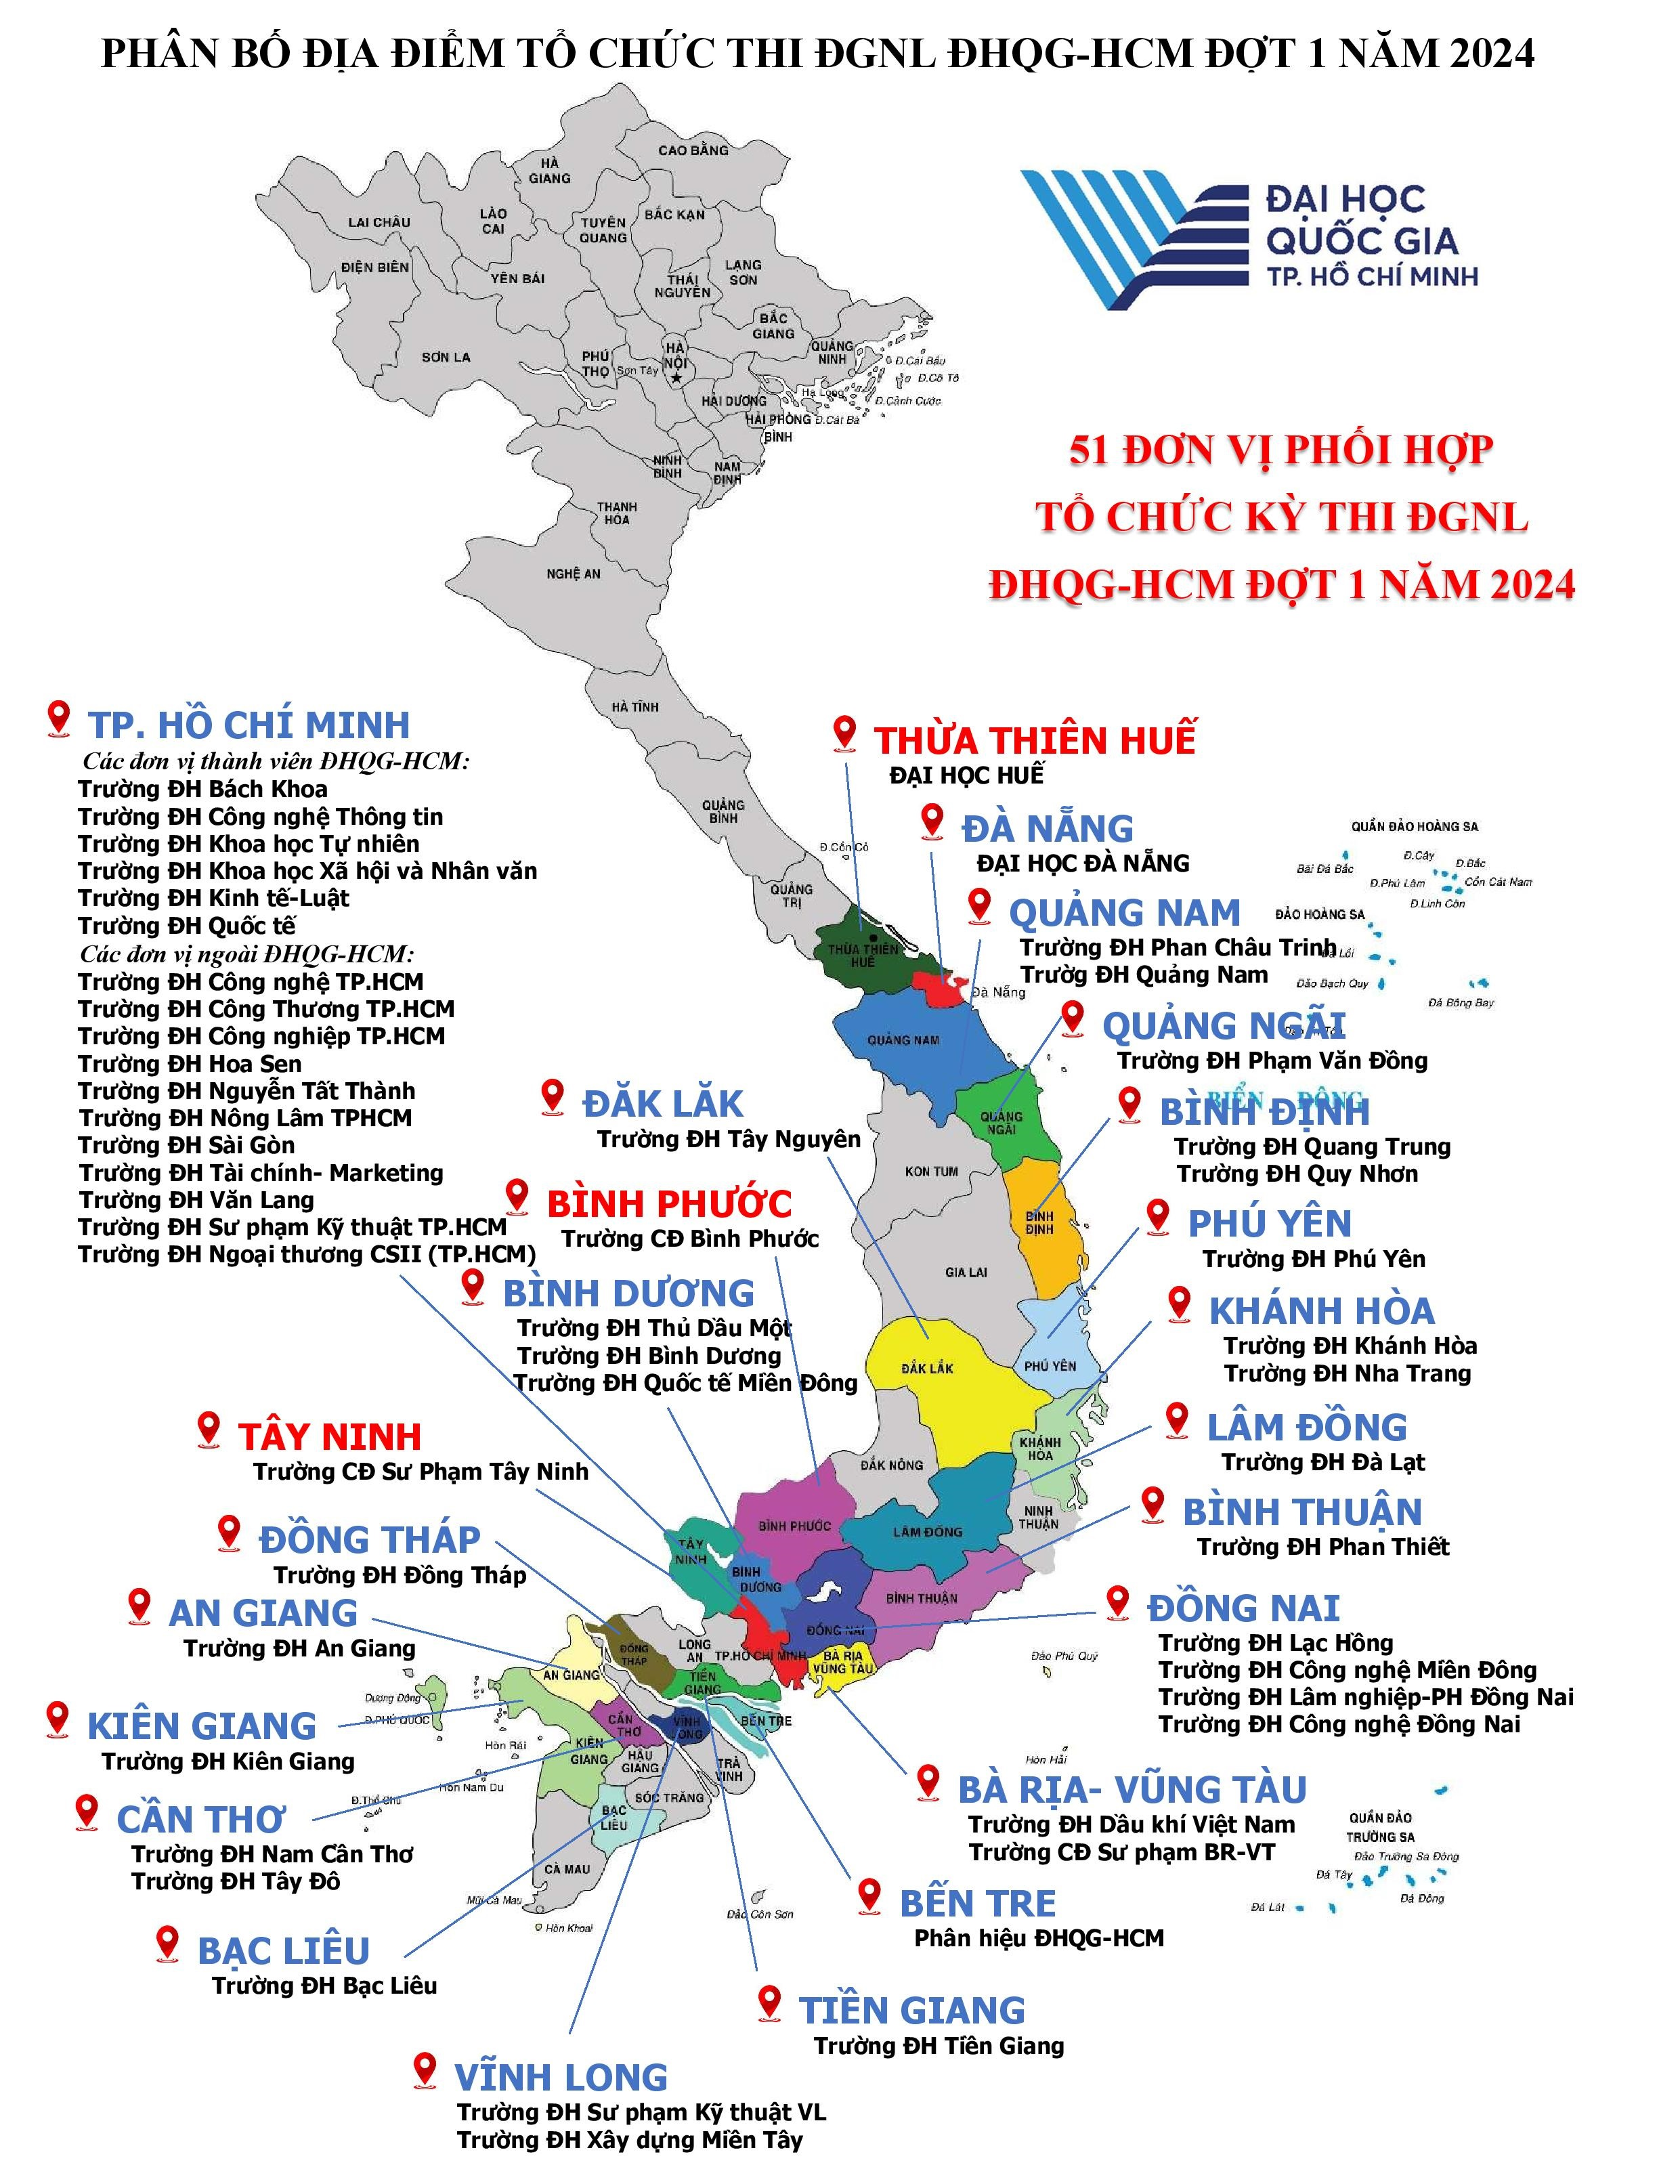
\includegraphics[width=1\linewidth]{img/Phan-bo-diem-thi-DGNL-Dot-1-2024.jpg}
    \caption{Phân bố điểm thi ĐGNL Đợt 1 - 2024}
    \label{fig:phanbodiemthi_dot1}
\end{figure}


\end{document}